\section{Simulating the Detector Electronics}

\subsection{Noise within IceCube-DeepCore}
The noise simulation module used in IceCube, known as \emph{Vuvuzela}, models the Poissonian and non-Poissonian detector noise using a set of five  parameters, each representing distinct processes \cite{Thesis-Vuvuzela, Description-IceCube}. 

The \emph{thermal noise} and \emph{radioactive decays} are Poisson processes simulated using rates fit during calibration.
The thermal rate is correlated with the temperature and forms a large component of the noise in IceCube DOMs, with a typical rate of 200 Hz while the decay rate has a typical value of 50-100 Hz due to radioactive activity in the DOM glass.

In order to model this bursting behavior described in Section~\ref{subsec:noise}, an effective model used which represents the timing of consecutive hits using a log-normal distribution. 
This introduces three additional parameters to the noise model: the average number of hits in a "burst", giving the normalization; the mean time between hits within a burst; and the standard deviation of the timing within a burst. 
The non-Poissonian component to the noise model produces an additional 400 Hz of noise \cite{Thesis-Vuvuzela}.
Noise hits in simulation are added as additional charge on each DOM at the face of the PMT.

The Vuvuzela model has previously been fit to each DOM in the detector, although with some limitations. 
Work completed during this thesis, discussed in Chapter~\ref{chapter:vuvuzela}, improved the calibration of the noise model.

\label{subsec:pmtsim}
\subsection{PMTResponseSimulator and DOMLauncher}
The IceCube detector does not directly measure photoelectrons emitted from the photocathode. 
Instead, IceCube events record the voltage response from the PMT via the output waveform.
The production of simulated waveforms from incident photons is produced by a pair of modules.

\begin{figure}
\centering
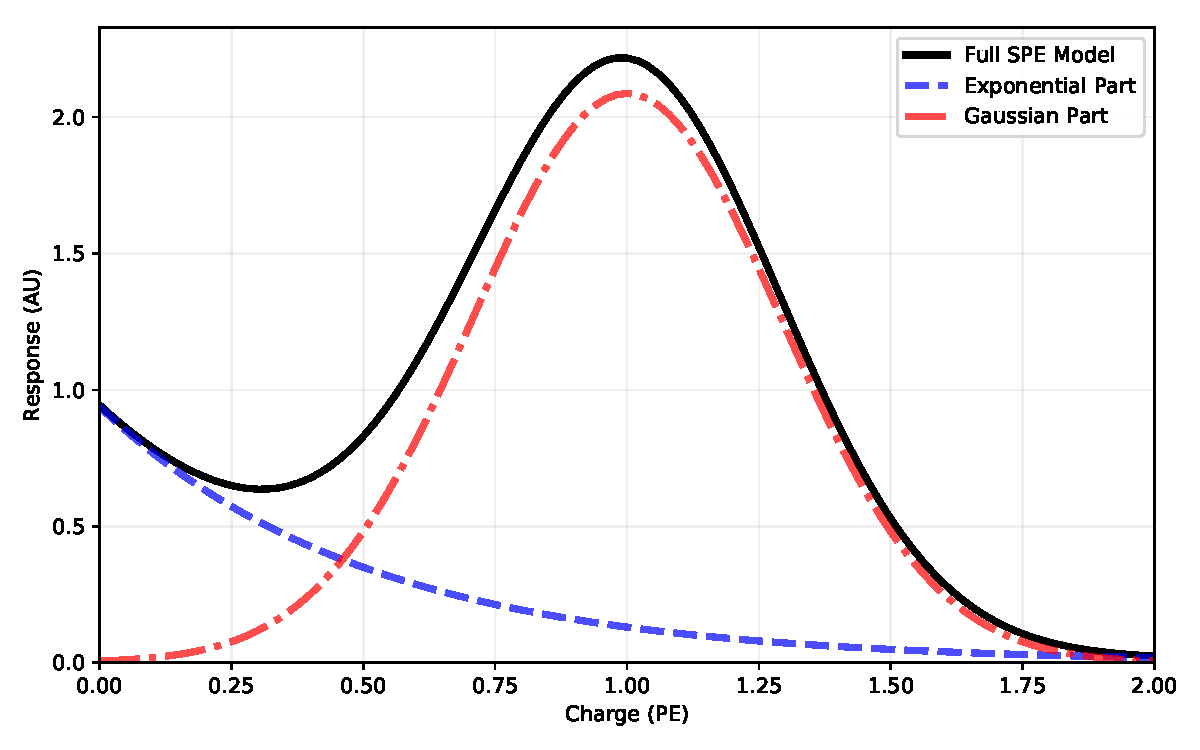
\includegraphics[width=0.7\textwidth]{ta0003.pdf} 
\caption{The SPE template used in Monte Carlo simulation. The gaussian (red, dash-dot) and exponential (blue, dashed) parts of the full model (black) are shown. The SPE template is used as a sampling distribution for each incident photon in order to determine the observed charge. The SPE template is used for all DOMs.}
\label{fig:ta0003}
\end{figure}

The first module, \emph{PMTResponseSimulator}, simulates the amplification process of the PMT, including the effects of pre-, late-, and afterpulsing.
Each of these three effects is modeled using calibration measurements performed in the lab \cite{IceCube-PMT}.
PMTResponseSimulator also calculates the amount of charge recorded by the DOM from each incident photon reaching the photocathode by sampling from the \emph{single photoelectron} template (\emph{SPE} template).
The SPE template used in simulation generation is calculated from lab measurements of 118 DOMs prior to deployment \cite{TA0003}.
The template, shown in Figure~\ref{fig:ta0003}, is represented by the sum of an exponential and gaussian term and is applied identically to all DOMs.

Prepulses, late pulses, and afterpulses are applied in a recursive process, which every incident hit having a probability of 0.3\%, 3.5\%, and 5.93\% to produce each respectively.
These probabilities were measured in the lab and are used for all DOMs. 

The second module, \emph{DOMLauncher}, handles the local coincidence circuits, simulation of the DOM clock, the discriminator, and digitization.
The triggering system is then applied following the description of Section~\ref{subsec:triggers}.
